
\chapter{Optimierung der Gangschaltung für höhere Geschwindigkeiten und kontinuierliches Mitfahren}


Die Anpassung der Gangschaltung und der Kettenplatten spielt eine entscheidende Rolle bei der Gewährleistung einer nahtlosen Fahrraderfahrung, insbesondere wenn höhere Geschwindigkeiten erreicht werden sollen. Das Ziel ist es, sicherzustellen, dass Sie auch bei erhöhter Geschwindigkeit noch bequem und effektiv mittreten können, um die optimale Leistung aus Ihrem E-Bike zu ziehen.\\

Hier sind einige Schritte und Überlegungen zur Anpassung der Gangschaltung:\\

    1. Mehr Gänge: Eine erweiterte Gangschaltung mit mehr Gängen ermöglicht eine feinere Abstimmung der Übersetzungen. Dadurch können Sie die passende Gangstufe wählen, um die Effizienz bei höheren Geschwindigkeiten zu steigern, ohne zu viel Kraft aufwenden zu müssen.\\

    2. Optimale Übersetzung: Die Auswahl der richtigen Kettenblätter und Ritzel ist entscheidend. Sie sollten eine Kombination wählen, die es Ihnen ermöglicht, bei hohen Geschwindigkeiten mit weniger Anstrengung zu treten. Dies verhindert ein zu schnelles "Ausdrehen" der Pedale und ermöglicht ein kontinuierliches Mitfahren.\\

    3. Testfahrten: Nach der Anpassung der Gangschaltung sollten ausgiebige Testfahrten durchgeführt werden. Auf diese Weise können Sie sicherstellen, dass die gewählten Einstellungen tatsächlich zu einem angenehmen Fahrerlebnis bei hohen Geschwindigkeiten führen.\\


\begin{figure}[h]
    \centering
    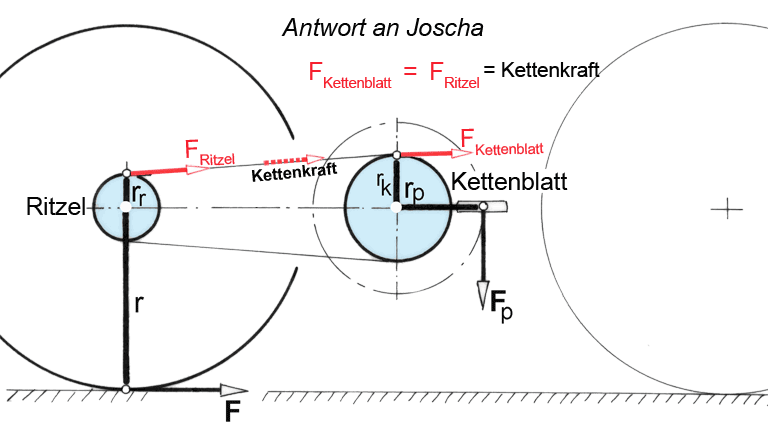
\includegraphics[width=8cm]{images/fahrrad_kraefte_gross.png}
    \caption{Meine Grafik}
    \label{fig:meine-grafik}
\end{figure}

Die richtige Anpassung der Gangschaltung und der Kettenplatten gewährleistet, dass Ihr E-Bike in verschiedenen Situationen und Geschwindigkeiten optimal funktioniert. Dies ermöglicht ein angenehmes Fahrerlebnis, bei dem Sie die elektrische Unterstützung nutzen können, ohne auf das Mitfahren verzichten zu müssen.\\

Im weiteren Verlauf Ihrer Studienarbeit werden wir weitere Schritte bei der Konstruktion und Anpassung Ihres selbstgebauten E-Bikes erkunden, einschließlich der Vorbereitung des Fahrrads auf erhöhte Kraftauswirkungen und der Integration aller Komponenten für eine reibungslose Fahrt.\\
%Die Gangschaltung und Kettenplätter sollen so angepasst werden das man auch bei hochen geschwindigkeiten noch mit treten kann.
